\begin{frame}
\frametitle{Operations: three kinds}

\begin{itemize}
  \item \textbf{\hh-BLAS1\&2:} Assembly, AXPY, GEMV \newline
        Simple. Operating only on leaves.
  \item \textbf{\hh-BLAS3:} GEMM, TRSV \newline 
        More involved. Operations at many different levels of the same sub-tree.
  \item \textbf{\hh-LAPACK:} Inverse, $LU$, $LL^T$.\newline
        Uses BLAS2 and BLAS3 operations, harder to implement in parallel.
\end{itemize}

\begin{block}{Base operations}
All operations use BLAS/LAPACK. Typical subroutines are: SVD, QR, 
LU, TRSV, GEMM and GEMV.
\end{block}
\end{frame}

%% Addition
\begin{frame}
\frametitle{Addition}
\begin{itemize}
  \item \textit{Usually} structures must be the same;
  \item 3 different base cases:
  \begin{itemize}
    \item sum of two dense matrices (usual dense operation);
    \item sum of a dense and a low-rank matrix;
    \item \textcolor{red}{sum of two low-rank matrices.}
  \end{itemize}
\end{itemize}
\begin{alert}{Useful pointers}
\begin{itemize}
\item Adding two low-rank matrices: unknown final rank
\item Costly operation!
\end{itemize}
\end{alert}
\end{frame}

%% From here: multiplication
\begin{frame}
\frametitle{Multiplication}

%% FROM
\only<1|handout:3>{

\begin{center}
\begin{tikzpicture}[scale=0.5]
  %% matrix A
  \draw[ thick] (0,0) rectangle (4.0,4.0);
  \draw[ thick] (0,0) rectangle (2.0,2.0);
  \draw[ thick] (2.0,2.0) rectangle (4.0,4.0);
    \draw[ thick] (2.0,2.0) rectangle (3.0,3.0);
    \draw[ thick] (3.0,3.0) rectangle (4.0,4.0);
    \draw[ thick] (2.0,4.0) rectangle (3.0,3.0);
    \draw[ thick] (3.0,3.0) rectangle (4.0,2.0);

  \draw[ thick] (0,4.0) rectangle (2.0,2.0);
  \draw[ thick] (2.0,2.0) rectangle (4.0,0.0);

  %% matrix L
  \draw[ thick] (5.0,0) rectangle (9.0,4.0);
  \draw[ thick] (5.0,0) rectangle (7.0,2.0);
    \draw[ thick] (5.0,0) rectangle (6.0,1.0);
    \draw[ thick] (6.0,1.0) rectangle (7.0,2.0);
    \draw[ thick] (7.0,0) rectangle (6.0,1.0);
    \draw[ thick] (6.0,1.0) rectangle (5.0,0.0);
  \draw[ thick] (7.0,2.0) rectangle (9.0,4.0);
  \draw[ thick] (5,4.0) rectangle (7.0,2.0);
  \draw[ thick] (7.0,2.0) rectangle (9.0,0.0);

  %% matrix L^T
  \draw[ thick] (10.0,0) rectangle (14.0,4.0);
  \draw[ thick] (10.0,0) rectangle (12.0,2.0);
  \draw[ thick] (12.0,2.0) rectangle (14.0,4.0);
    \draw[ thick] (12.0,2.0) rectangle (13.0,3.0);
    \draw[ thick] (13.0,3.0) rectangle (14.0,4.0);
    \draw[ thick] (12.0,4.0) rectangle (13.0,3.0);
    \draw[ thick] (13.0,3.0) rectangle (14.0,2.0);


  \draw[ thick] (10.0,4.0) rectangle (12.0,2.0);
  \draw[ thick] (12.0,2.0) rectangle (14.0,0.0);

  \filldraw[fill=cyan, draw=blue] (10.0,0.0) rectangle (14.0,4.0);
  \node[fontsize=14] at (12.0, 2.0) {?};

  \node at (4.5,2.0) {$\times$};
  \node at (9.5,2.0) {$=$};

  \node[below] at (12.0,0.0) {$C$};
  \node[below] at (7.0,0.0) {$B$};
  \node[below] at (2.0,0.0) {$A$};

\end{tikzpicture}
\end{center}

\begin{block}{Main issues}
Let $C= A \times B$ the product of 2 \hmats. 
\begin{itemize}
\item \textcolor{red}{What is the 'best' structure of C ?}
\item Uniqueness ?
\item What if it is imposed ?
\end{itemize}
\end{block}
}
\only<2|handout:3>{

\begin{center}
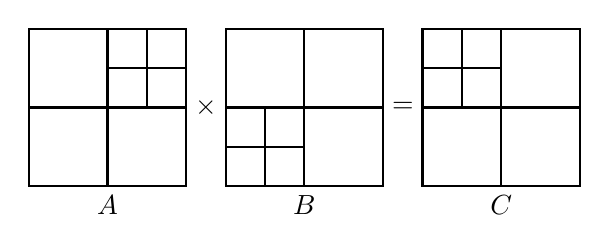
\begin{tikzpicture}[scale=0.5]
  %% matrix A
  \draw[ thick] (0,0) rectangle (4.0,4.0);
  \draw[ thick] (0,0) rectangle (2.0,2.0);
  \draw[ thick] (2.0,2.0) rectangle (4.0,4.0);
    \draw[ thick] (2.0,2.0) rectangle (3.0,3.0);
    \draw[ thick] (3.0,3.0) rectangle (4.0,4.0);
    \draw[ thick] (2.0,4.0) rectangle (3.0,3.0);
    \draw[ thick] (3.0,3.0) rectangle (4.0,2.0);
  \draw[ thick] (0,4.0) rectangle (2.0,2.0);
  \draw[ thick] (2.0,2.0) rectangle (4.0,0.0);

  %% matrix L
  \draw[ thick] (5.0,0) rectangle (9.0,4.0);
  \draw[ thick] (5.0,0) rectangle (7.0,2.0);
    \draw[ thick] (5.0,0) rectangle (6.0,1.0);
    \draw[ thick] (6.0,1.0) rectangle (7.0,2.0);
    \draw[ thick] (7.0,0) rectangle (6.0,1.0);
    \draw[ thick] (6.0,1.0) rectangle (5.0,0.0);
  \draw[ thick] (7.0,2.0) rectangle (9.0,4.0);
  \draw[ thick] (5,4.0) rectangle (7.0,2.0);
  \draw[ thick] (7.0,2.0) rectangle (9.0,0.0);

  %% matrix L^T
  \draw[ thick] (10.0,0) rectangle (14.0,4.0);
    \draw[ thick] (10.0,0) rectangle (12.0,2.0);
    \draw[ thick] (12.0,2.0) rectangle (14.0,4.0);
    \draw[ thick] (10.0,4.0) rectangle (12.0,2.0);
      \draw[thick] (10.0,4.0) rectangle (11.0,3.0);
      \draw[thick] (11.0,3.0) rectangle (10.0,2.0);
      \draw[thick] (10.0,2.0) rectangle (11.0,3.0);
      \draw[thick] (11.0,3.0) rectangle (12.0,4.0);

    \draw[ thick] (12.0,2.0) rectangle (14.0,0.0);


  %% A
  \node at (4.5,2.0) {$\times$};
  \node at (9.5,2.0) {$=$};
  \node[below] at (12.0,0.0) {$C$};
  \node[below] at (7.0,0.0) {$B$};
  \node[below] at (2.0,0.0) {$A$};

\end{tikzpicture}
\end{center}

\begin{block}{Main issues}
Let $C= A \times B$ the product of 2 \hmats. 
\begin{itemize}
\item What is the 'best' structure of C ?
\item \textcolor{red}{Uniqueness ? (here the literature definition)}
\item What if it is imposed ?
\end{itemize}
\end{block}

}
\only<3|handout:3>{

\begin{center}
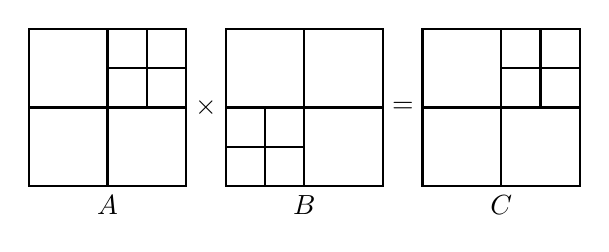
\begin{tikzpicture}[scale=0.5]
  %% matrix A
  \draw[ thick] (0,0) rectangle (4.0,4.0);
  \draw[ thick] (0,0) rectangle (2.0,2.0);
  \draw[ thick] (2.0,2.0) rectangle (4.0,4.0);
    \draw[ thick] (2.0,2.0) rectangle (3.0,3.0);
    \draw[ thick] (3.0,3.0) rectangle (4.0,4.0);
    \draw[ thick] (2.0,4.0) rectangle (3.0,3.0);
    \draw[ thick] (3.0,3.0) rectangle (4.0,2.0);
  \draw[ thick] (0,4.0) rectangle (2.0,2.0);
  \draw[ thick] (2.0,2.0) rectangle (4.0,0.0);

  %% matrix L
  \draw[ thick] (5.0,0) rectangle (9.0,4.0);
  \draw[ thick] (5.0,0) rectangle (7.0,2.0);
    \draw[ thick] (5.0,0) rectangle (6.0,1.0);
    \draw[ thick] (6.0,1.0) rectangle (7.0,2.0);
    \draw[ thick] (7.0,0) rectangle (6.0,1.0);
    \draw[ thick] (6.0,1.0) rectangle (5.0,0.0);
  \draw[ thick] (7.0,2.0) rectangle (9.0,4.0);
  \draw[ thick] (5,4.0) rectangle (7.0,2.0);
  \draw[ thick] (7.0,2.0) rectangle (9.0,0.0);

  %% matrix L^T
  \draw[ thick] (10.0,0) rectangle (14.0,4.0);
  \draw[ thick] (10.0,0) rectangle (12.0,2.0);
  \draw[ thick] (12.0,2.0) rectangle (14.0,4.0);
    \draw[ thick] (12.0,2.0) rectangle (13.0,3.0);
    \draw[ thick] (13.0,3.0) rectangle (14.0,4.0);
    \draw[ thick] (12.0,4.0) rectangle (13.0,3.0);
    \draw[ thick] (13.0,3.0) rectangle (14.0,2.0);
  \draw[ thick] (10.0,4.0) rectangle (12.0,2.0);
  \draw[ thick] (12.0,2.0) rectangle (14.0,0.0);

  %% A
  \node at (4.5,2.0) {$\times$};
  \node at (9.5,2.0) {$=$};
  \node[below] at (12.0,0.0) {$C$};
  \node[below] at (7.0,0.0) {$B$};
  \node[below] at (2.0,0.0) {$A$};

\end{tikzpicture}
\end{center}

\begin{block}{Main issues}
Let $C= A \times B$ the product of 2 \hmats. 
\begin{itemize}
\item What is the 'best' structure of C ?
\item Uniqueness ?
\item \textcolor{red}{What if it is imposed ? (e.g. in a $LL^T$ factorization)}
\end{itemize}
\end{block}
}
\end{frame}

%% begin GEMM
\begin{frame}
\frametitle{Multiplication: exemple 1}
\only<1|handout:2>{
  
\begin{center}
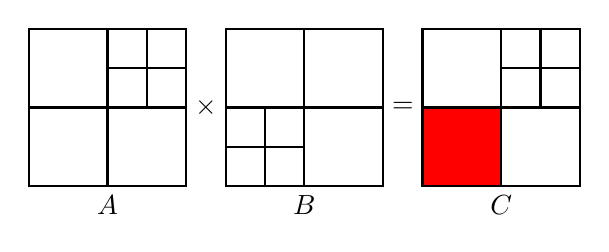
\begin{tikzpicture}[scale=0.5]
  %% matrix A
  \draw[ thick] (0,0) rectangle (4.0,4.0);
  \draw[ thick] (0,0) rectangle (2.0,2.0);
  \draw[ thick] (2.0,2.0) rectangle (4.0,4.0);
    \draw[ thick] (2.0,2.0) rectangle (3.0,3.0);
    \draw[ thick] (3.0,3.0) rectangle (4.0,4.0);
    \draw[ thick] (2.0,4.0) rectangle (3.0,3.0);
    \draw[ thick] (3.0,3.0) rectangle (4.0,2.0);
  \draw[ thick] (0,4.0) rectangle (2.0,2.0);
  \draw[ thick] (2.0,2.0) rectangle (4.0,0.0);

  %% matrix B
  \draw[ thick] (5.0,0) rectangle (9.0,4.0);
  \draw[ thick] (5.0,0) rectangle (7.0,2.0);
    \draw[ thick] (5.0,0) rectangle (6.0,1.0);
    \draw[ thick] (6.0,1.0) rectangle (7.0,2.0);
    \draw[ thick] (7.0,0) rectangle (6.0,1.0);
    \draw[ thick] (6.0,1.0) rectangle (5.0,0.0);
  \draw[ thick] (7.0,2.0) rectangle (9.0,4.0);
  \draw[ thick] (5,4.0) rectangle (7.0,2.0);
  \draw[ thick] (7.0,2.0) rectangle (9.0,0.0);

  %% matrix C
  \filldraw[ fill=red, draw=black] (10.0,0.0) rectangle (12.0,2.0);
  \draw[thick] (10.0,0) rectangle (14.0,4.0);
  \draw[thick] (10.0,0) rectangle (12.0,2.0);
  \draw[thick] (12.0,2.0) rectangle (14.0,4.0);
    \draw[thick] (12.0,2.0) rectangle (13.0,3.0);
    \draw[thick] (13.0,3.0) rectangle (14.0,4.0);
    \draw[thick] (12.0,4.0) rectangle (13.0,3.0);
    \draw[thick] (13.0,3.0) rectangle (14.0,2.0);
  \draw[thick] (10.0,4.0) rectangle (12.0,2.0);
  \draw[thick] (12.0,2.0) rectangle (14.0,0.0);

  %% A
  \node at (4.5,2.0) {$\times$};
  \node at (9.5,2.0) {$=$};
  \node[below] at (12.0,0.0) {$C$};
  \node[below] at (7.0,0.0) {$B$};
  \node[below] at (2.0,0.0) {$A$};

\end{tikzpicture}
\end{center}


}
\only<2|handout:2>{
  \begin{center}
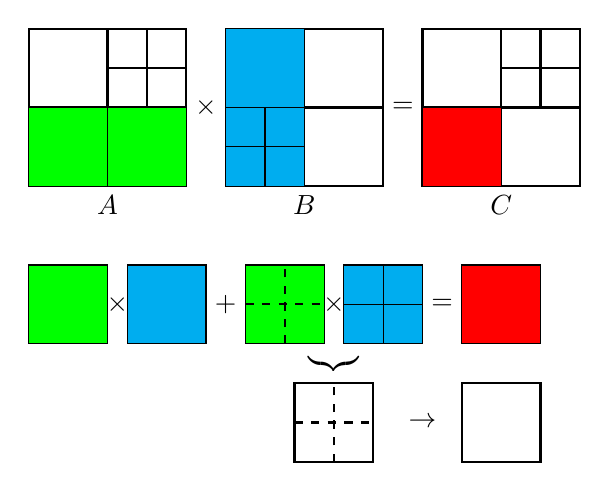
\begin{tikzpicture}[scale=0.5]
  %% matrix A
  \draw[ thick] (0,0) rectangle (4.0,4.0);
  \draw[ thick] (0,0) rectangle (2.0,2.0);
  \draw[ thick] (2.0,2.0) rectangle (4.0,4.0);
    \draw[ thick] (2.0,2.0) rectangle (3.0,3.0);
    \draw[ thick] (3.0,3.0) rectangle (4.0,4.0);
    \draw[ thick] (2.0,4.0) rectangle (3.0,3.0);
    \draw[ thick] (3.0,3.0) rectangle (4.0,2.0);
  \draw[ thick] (0,4.0) rectangle (2.0,2.0);
  \draw[ thick] (2.0,2.0) rectangle (4.0,0.0);


    \filldraw[fill=green, draw=black] (0.0,0.0) rectangle (2.0,2.0);
    \filldraw[fill=green, draw=black] (2.0,0.0) rectangle (4.0,2.0);

  %% matrix B
  \draw[ thick] (5.0,0) rectangle (9.0,4.0);
  \draw[ thick] (5.0,0) rectangle (7.0,2.0);
    \draw[ thick] (5.0,0) rectangle (6.0,1.0);
    \draw[ thick] (6.0,1.0) rectangle (7.0,2.0);
    \draw[ thick] (7.0,0) rectangle (6.0,1.0);
    \draw[ thick] (6.0,1.0) rectangle (5.0,0.0);
  \draw[ thick] (7.0,2.0) rectangle (9.0,4.0);
  \draw[ thick] (5,4.0) rectangle (7.0,2.0);
  \draw[ thick] (7.0,2.0) rectangle (9.0,0.0);

  \filldraw[fill=cyan, draw=black] (5,4.0) rectangle (7.0,2.0);
    \filldraw[fill=cyan, draw=black] (5.0,2.0) rectangle (6.0,1.0);
    \filldraw[fill=cyan, draw=black] (6.0,1.0) rectangle (7.0,2.0);
    \filldraw[fill=cyan, draw=black] (7.0,0) rectangle (6.0,1.0);
    \filldraw[fill=cyan, draw=black] (6.0,1.0) rectangle (5.0,0.0);

  %% matrix C
  \draw[thick] (10.0,0) rectangle (14.0,4.0);
  \draw[thick] (10.0,0) rectangle (12.0,2.0);
  \draw[thick] (12.0,2.0) rectangle (14.0,4.0);
    \draw[thick] (12.0,2.0) rectangle (13.0,3.0);
    \draw[thick] (13.0,3.0) rectangle (14.0,4.0);
    \draw[thick] (12.0,4.0) rectangle (13.0,3.0);
    \draw[thick] (13.0,3.0) rectangle (14.0,2.0);
  \draw[thick] (10.0,4.0) rectangle (12.0,2.0);
  \draw[thick] (12.0,2.0) rectangle (14.0,0.0);
  \filldraw[ fill=red, draw=black] (10.0,0.0) rectangle (12.0,2.0);

  %% A
  \node at (4.5,2.0) {$\times$};
  \node at (9.5,2.0) {$=$};
  \node[below] at (12.0,0.0) {$C$};
  \node[below] at (7.0,0.0) {$B$};
  \node[below] at (2.0,0.0) {$A$};

  \filldraw[fill=green, draw=black] (0.0,-4.0) rectangle (2.0,-2.0);
  \filldraw[fill=cyan, draw=black] (2.5,-4.0) rectangle (4.5,-2.0);

  \filldraw[fill=green, draw=black] (5.5,-4.0) rectangle (7.5,-2.0);
    \draw[dashed, thick] (6.5,-4.0) -- (6.5,-2.0);
    \draw[dashed, thick] (5.5,-3.0) -- (7.5,-3.0);

  \filldraw[fill=cyan, draw=black] (8.0,-4.0) rectangle (10.0,-2.0);
    \filldraw[fill=cyan, draw=black] (8.0,-4.0) rectangle (9.0,-3.0);
    \filldraw[fill=cyan, draw=black] (9.0,-3.0) rectangle (10.0,-2.0);
    \filldraw[fill=cyan, draw=black] (8.0,-2.0) rectangle (9.0,-3.0);
    \filldraw[fill=cyan, draw=black] (9.0,-3.0) rectangle (10.0,-4.0);

  \node at (2.25,-3) {$\times$};
  \node at (5.0,-3) {$+$};
  \node at (7.75,-3) {$\times$};
  \node[below] at (7.75,-4) {$\underbrace{}$};

  \node at (10.5,-3) {$=$};
  \filldraw[fill=red, draw=black] (11.0,-4.0) rectangle (13.0,-2.0);

  \draw[thick] (6.75,-7.0) rectangle (8.75,-5.0);
  \draw[dashed, thick] (7.75,-7.0) -- (7.75,-5.0);
  \draw[dashed, thick] (6.75,-6.0) -- (8.75,-6.0);

  \draw[thick] (11.0,-7.0) rectangle (13.0,-5.0);
  \node at (10.0,-6.0) {$\rightarrow$};

\end{tikzpicture}
\end{center}


}
\end{frame}

\begin{frame}
\frametitle{Multiplication: exemple 2}
\only<1|handout:2>{
  
\begin{center}
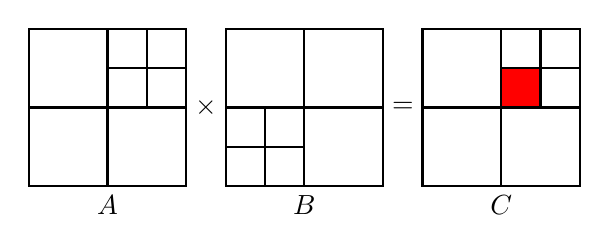
\begin{tikzpicture}[scale=0.5]
  %% matrix A
  \draw[ thick] (0,0) rectangle (4.0,4.0);
  \draw[ thick] (0,0) rectangle (2.0,2.0);
  \draw[ thick] (2.0,2.0) rectangle (4.0,4.0);
    \draw[ thick] (2.0,2.0) rectangle (3.0,3.0);
    \draw[ thick] (3.0,3.0) rectangle (4.0,4.0);
    \draw[ thick] (2.0,4.0) rectangle (3.0,3.0);
    \draw[ thick] (3.0,3.0) rectangle (4.0,2.0);
  \draw[ thick] (0,4.0) rectangle (2.0,2.0);
  \draw[ thick] (2.0,2.0) rectangle (4.0,0.0);

  %% matrix B
  \draw[ thick] (5.0,0) rectangle (9.0,4.0);
  \draw[ thick] (5.0,0) rectangle (7.0,2.0);
    \draw[ thick] (5.0,0) rectangle (6.0,1.0);
    \draw[ thick] (6.0,1.0) rectangle (7.0,2.0);
    \draw[ thick] (7.0,0) rectangle (6.0,1.0);
    \draw[ thick] (6.0,1.0) rectangle (5.0,0.0);
  \draw[ thick] (7.0,2.0) rectangle (9.0,4.0);
  \draw[ thick] (5,4.0) rectangle (7.0,2.0);
  \draw[ thick] (7.0,2.0) rectangle (9.0,0.0);

  %% matrix C
  \filldraw[ fill=red, draw=black] (12.0,2.0) rectangle (13.0,3.0);
  \draw[thick] (10.0,0) rectangle (14.0,4.0);
  \draw[thick] (10.0,0) rectangle (12.0,2.0);
  \draw[thick] (12.0,2.0) rectangle (14.0,4.0);
    \draw[thick] (12.0,2.0) rectangle (13.0,3.0);
    \draw[thick] (13.0,3.0) rectangle (14.0,4.0);
    \draw[thick] (12.0,4.0) rectangle (13.0,3.0);
    \draw[thick] (13.0,3.0) rectangle (14.0,2.0);
  \draw[thick] (10.0,4.0) rectangle (12.0,2.0);
  \draw[thick] (12.0,2.0) rectangle (14.0,0.0);

  %% A
  \node at (4.5,2.0) {$\times$};
  \node at (9.5,2.0) {$=$};
  \node[below] at (12.0,0.0) {$C$};
  \node[below] at (7.0,0.0) {$B$};
  \node[below] at (2.0,0.0) {$A$};

\end{tikzpicture}
\end{center}

}
\only<2|handout:2>{
  %% exemple of a matrix/matrix product in hmat
\begin{center}
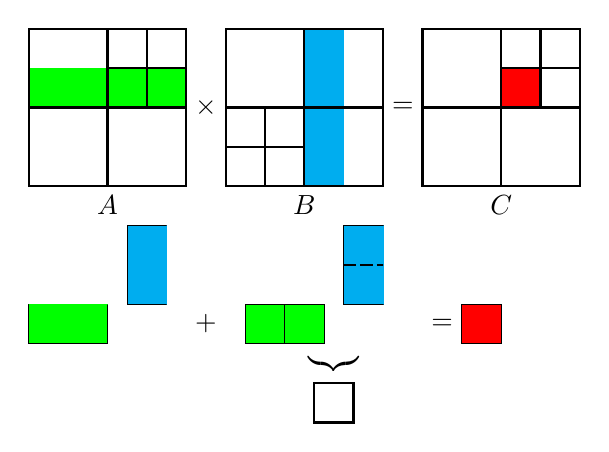
\begin{tikzpicture}[scale=0.5]
  %% matrix A
  \filldraw[fill=green, draw=green] (0,2) rectangle (2,3);
  \filldraw[fill=green, draw=green] (2,2) rectangle (3,3);
  \filldraw[fill=green, draw=green] (3,2) rectangle (4,3);
  
  \draw[ thick] (0,0) rectangle (4.0,4.0);
  \draw[ thick] (0,0) rectangle (2.0,2.0);
  \draw[ thick] (2.0,2.0) rectangle (4.0,4.0);
    \draw[ thick] (2.0,2.0) rectangle (3.0,3.0);
    \draw[ thick] (3.0,3.0) rectangle (4.0,4.0);
    \draw[ thick] (2.0,4.0) rectangle (3.0,3.0);
    \draw[ thick] (3.0,3.0) rectangle (4.0,2.0);
  \draw[ thick] (0,4.0) rectangle (2.0,2.0);
  \draw[ thick] (2.0,2.0) rectangle (4.0,0.0);

  %% matrix B
  \filldraw[fill=cyan, draw=cyan] (7.0,2.0) rectangle (8.0,4.0);
  \filldraw[fill=cyan, draw=cyan] (7.0,0.0) rectangle (8.0,2.0);
  \draw[ thick] (5.0,0) rectangle (9.0,4.0);
  \draw[ thick] (5.0,0) rectangle (7.0,2.0);
    \draw[ thick] (5.0,0) rectangle (6.0,1.0);
    \draw[ thick] (6.0,1.0) rectangle (7.0,2.0);
    \draw[ thick] (7.0,0) rectangle (6.0,1.0);
    \draw[ thick] (6.0,1.0) rectangle (5.0,0.0);
  \draw[ thick] (7.0,2.0) rectangle (9.0,4.0);
  \draw[ thick] (5,4.0) rectangle (7.0,2.0);
  \draw[ thick] (7.0,2.0) rectangle (9.0,0.0);

  %% matrix C
  \draw[thick] (10.0,0) rectangle (14.0,4.0);
  \draw[thick] (10.0,0) rectangle (12.0,2.0);
  \draw[thick] (12.0,2.0) rectangle (14.0,4.0);
    \draw[thick] (12.0,2.0) rectangle (13.0,3.0);
      \filldraw[fill=red, draw=black] (12.0,2.0) rectangle (13.0,3.0);
    \draw[thick] (13.0,3.0) rectangle (14.0,4.0);
    \draw[thick] (12.0,4.0) rectangle (13.0,3.0);
    \draw[thick] (13.0,3.0) rectangle (14.0,2.0);
  \draw[thick] (10.0,4.0) rectangle (12.0,2.0);
  \draw[thick] (12.0,2.0) rectangle (14.0,0.0);

  %% A
  \node at (4.5,2.0) {$\times$};
  \node at (9.5,2.0) {$=$};
  \node[below] at (12.0,0.0) {$C$};
  \node[below] at (7.0,0.0) {$B$};
  \node[below] at (2.0,0.0) {$A$};

  \filldraw[fill=cyan, draw=black] (8.0,-3.0) rectangle (9.0,-1.0);
  \draw[cyan] (9.0,-3.0) rectangle (9.0,-1.0);
  \draw[dashed] (8.0,-2.0) rectangle (9.0,-2.0);

  \node at (4.5,-3.5) {$+$};
  \node[below] at (7.75,-4) {$\underbrace{}$};

  \node at (10.5,-3.5) {$=$};
  \filldraw[fill=red, draw=black] (11.0,-4.0) rectangle (12.0,-3.0);
  \draw[thick] (7.25,-6.0) rectangle (8.25,-5.0);


  \filldraw[fill=green, draw=black] (0,-4) rectangle (2,-3);
  \draw[fill=green, draw=black] (0,-4) rectangle (2,-3);
  \draw[green] (0,-3) rectangle (2,-3);
  \filldraw[fill=cyan, draw=black] (2.5,-3.0) rectangle (3.5,-1.0);
  \draw[draw=cyan] (3.5,-3.0) rectangle (3.5,-1.0);

  \filldraw[fill=green, draw=black] (5.5,-4) rectangle (6.5,-3);
  \filldraw[fill=green, draw=black] (6.5,-4) rectangle (7.5,-3);

\end{tikzpicture}
\end{center}


}
\end{frame}
%% end GEMM

%% begin CHOLESKY
\begin{frame}
\frametitle{Cholesky factorization}
%%
Recall: recursive block splitting based on the $2 \times 2$ block structure.
\only<1|handout:4>{
\begin{center}
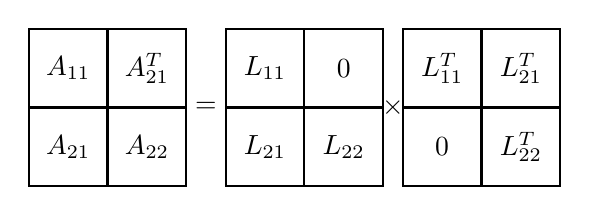
\begin{tikzpicture}[scale=0.5]
  %% matrix A
  \draw[ thick] (0,0) rectangle (4.0,4.0);
  \draw[ thick] (0,0) rectangle (2.0,2.0);
  \draw[ thick] (2.0,2.0) rectangle (4.0,4.0);
  \draw[ thick] (0,4.0) rectangle (2.0,2.0);
  %\filldraw[fill=cyan, draw=black] (0,4.0) rectangle (2.0,2.0);
  \draw[ thick] (2.0,2.0) rectangle (4.0,0.0);

  %% matrix L
  \draw[ thick] (5.0,0) rectangle (9.0,4.0);
  \draw[ thick] (5.0,0) rectangle (7.0,2.0);
  \draw[ thick] (7.0,2.0) rectangle (9.0,4.0);
  \draw[ thick] (5,4.0) rectangle (7.0,2.0);
  %\filldraw[fill=cyan, draw=black] (5,4.0) rectangle (7.0,2.0);
  \draw[ thick] (7.0,2.0) rectangle (9.0,0.0);

  %% matrix L^T
  \draw[ thick] (9.5,0) rectangle (13.50,4.0);
  \draw[ thick] (9.50,0) rectangle (11.50,2.0);
  \draw[ thick] (11.50,2.0) rectangle (13.50,4.0);
  \draw[ thick] (9.5,4.0) rectangle (11.50,2.0);
  %\filldraw[fill=cyan, draw=black] (9.5,4.0) rectangle (11.50,2.0);
  \draw[ thick] (11.50,2.0) rectangle (13.50,0.0);

  %% A
  \node at (1.,3.0) {$A_{11}$};
  \node at (3.,3.0) {$A_{21}^T$};
  \node at (1.,1.0) {$A_{21}$};
  \node at (3.,1.0) {$A_{22}$};


  \node at (4.5,2.0) {$=$};
  \node at (9.25,2.0) {$\times$};

  %% L
  \node at (8.,3.0) {$0$};
  \node at (6.,3.0) {$L_{11}$};
  \node at (6.,1.0) {$L_{21}$};
  \node at (8.,1.0) {$L_{22}$};

  %% L^T
  \node at (10.50,1.0) {$0$};
  \node at (10.50,3.0) {$L_{11}^T$};
  \node at (12.50,1.0) {$L_{22}^T$};
  \node at (12.50,3.0) {$L_{21}^T$};

\end{tikzpicture}
\end{center}

\begin{eqnarray*}
A_{11} & = & L_{11}L_{11}^T \\
A_{21} & = & L_{21}L_{11}^T  \\
A_{22} & = & L_{21}L_{21}^T + L_{22}L_{22}^T  
\end{eqnarray*}
}

\only<2|handout:4>{

%% image
\begin{center}
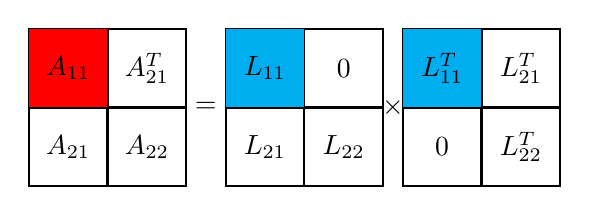
\begin{tikzpicture}[scale=0.5]
  %% matrix A
  \draw[ thick] (0,0) rectangle (4.0,4.0);
  \draw[ thick] (0,0) rectangle (2.0,2.0);
  \draw[ thick] (2.0,2.0) rectangle (4.0,4.0);
  \draw[ thick] (0,4.0) rectangle (2.0,2.0);
  \draw[ thick] (2.0,2.0) rectangle (4.0,0.0);

  %% matrix L
  \draw[ thick] (5.0,0) rectangle (9.0,4.0);
  \draw[ thick] (5.0,0) rectangle (7.0,2.0);
  \draw[ thick] (7.0,2.0) rectangle (9.0,4.0);
  \draw[ thick] (5,4.0) rectangle (7.0,2.0);
  \draw[ thick] (7.0,2.0) rectangle (9.0,0.0);

  %% matrix L^T
  \draw[ thick] (9.5,0) rectangle (13.50,4.0);
  \draw[ thick] (9.50,0) rectangle (11.50,2.0);
  \draw[ thick] (11.50,2.0) rectangle (13.50,4.0);
  \draw[ thick] (9.5,4.0) rectangle (11.50,2.0);
  \draw[ thick] (11.50,2.0) rectangle (13.50,0.0);

  %% highlights
  \filldraw[fill=red, draw=black] (0,4.0) rectangle (2.0,2.0);
  \filldraw[fill=cyan, draw=black] (5,4.0) rectangle (7.0,2.0);
  \filldraw[fill=cyan, draw=black] (9.5,4.0) rectangle (11.50,2.0);

  %% A
  \node at (1.,3.0) {$A_{11}$};
  \node at (3.,3.0) {$A_{21}^T$};
  \node at (1.,1.0) {$A_{21}$};
  \node at (3.,1.0) {$A_{22}$};


  \node at (4.5,2.0) {$=$};
  \node at (9.25,2.0) {$\times$};

  %% L
  \node at (8.,3.0) {$0$};
  \node at (6.,3.0) {$L_{11}$};
  \node at (6.,1.0) {$L_{21}$};
  \node at (8.,1.0) {$L_{22}$};

  %% L^T
  \node at (10.50,1.0) {$0$};
  \node at (10.50,3.0) {$L_{11}^T$};
  \node at (12.50,1.0) {$L_{22}^T$};
  \node at (12.50,3.0) {$L_{21}^T$};

\end{tikzpicture}
\end{center}
%%
\begin{eqnarray*}
\textcolor{red}{A_{11}} & = & \textcolor{blue} {L_{11}L_{11}^T} \qquad \text{(recursive call)} \\
A_{21} & = & L_{21}L_{11}^T \\ 
A_{22} & = & L_{21}L_{21}^T + L_{22}L_{22}^T 
\end{eqnarray*}
}

\only<3|handout:4>{

%% image
\begin{center}
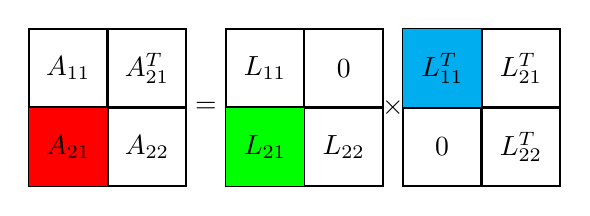
\begin{tikzpicture}[scale=0.5]
  %% matrix A
  \draw[ thick] (0,0) rectangle (4.0,4.0);
  \draw[ thick] (0,0) rectangle (2.0,2.0);
  \draw[ thick] (2.0,2.0) rectangle (4.0,4.0);
  \draw[ thick] (0,4.0) rectangle (2.0,2.0);
  \draw[ thick] (2.0,2.0) rectangle (4.0,0.0);

  %% matrix L
  \draw[ thick] (5.0,0) rectangle (9.0,4.0);
  \draw[ thick] (5.0,0) rectangle (7.0,2.0);
  \draw[ thick] (7.0,2.0) rectangle (9.0,4.0);
  \draw[ thick] (5,4.0) rectangle (7.0,2.0);
  \draw[ thick] (7.0,2.0) rectangle (9.0,0.0);

  %% matrix L^T
  \draw[ thick] (9.5,0) rectangle (13.50,4.0);
  \draw[ thick] (9.50,0) rectangle (11.50,2.0);
  \draw[ thick] (11.50,2.0) rectangle (13.50,4.0);
  \draw[ thick] (9.5,4.0) rectangle (11.50,2.0);
  \draw[ thick] (11.50,2.0) rectangle (13.50,0.0);

  %% highlights
  \filldraw[fill=red, draw=black] (0.0,0.0) rectangle (2.0,2.0);
  \filldraw[fill=green, draw=black] (5,0.0) rectangle (7.0,2.0);
  \filldraw[fill=cyan, draw=black] (9.5,4.0) rectangle (11.50,2.0);

  %% A
  \node at (1.,3.0) {$A_{11}$};
  \node at (3.,3.0) {$A_{21}^T$};
  \node at (1.,1.0) {$A_{21}$};
  \node at (3.,1.0) {$A_{22}$};


  \node at (4.5,2.0) {$=$};
  \node at (9.25,2.0) {$\times$};

  %% L
  \node at (8.,3.0) {$0$};
  \node at (6.,3.0) {$L_{11}$};
  \node at (6.,1.0) {$L_{21}$};
  \node at (8.,1.0) {$L_{22}$};

  %% L^T
  \node at (10.50,1.0) {$0$};
  \node at (10.50,3.0) {$L_{11}^T$};
  \node at (12.50,1.0) {$L_{22}^T$};
  \node at (12.50,3.0) {$L_{21}^T$};

\end{tikzpicture}
\end{center}
%%
\begin{eqnarray*}
A_{11} & = & L_{11}L_{11}^T \\
\textcolor{red}{A_{21}} & = & \textcolor{green}{L_{21}} \textcolor{blue}{L_{11}^T} \qquad \text{(upper triangular solve)} \\
A_{22} & = & L_{21}L_{21}^T + L_{22}L_{22}^T 
\end{eqnarray*}
}
%%

%%
\only<4|handout:4>{

%% image
\begin{center}
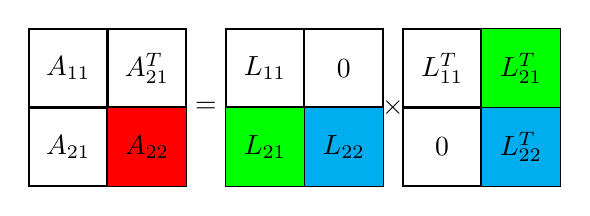
\begin{tikzpicture}[scale=0.5]
  %% matrix A
  \draw[ thick] (0,0) rectangle (4.0,4.0);
  \draw[ thick] (0,0) rectangle (2.0,2.0);
  \draw[ thick] (2.0,2.0) rectangle (4.0,4.0);
  \draw[ thick] (0,4.0) rectangle (2.0,2.0);
  \draw[ thick] (2.0,2.0) rectangle (4.0,0.0);

  %% matrix L
  \draw[ thick] (5.0,0) rectangle (9.0,4.0);
  \draw[ thick] (5.0,0) rectangle (7.0,2.0);
  \draw[ thick] (7.0,2.0) rectangle (9.0,4.0);
  \draw[ thick] (5,4.0) rectangle (7.0,2.0);
  \draw[ thick] (7.0,2.0) rectangle (9.0,0.0);

  %% matrix L^T
  \draw[ thick] (9.5,0) rectangle (13.50,4.0);
  \draw[ thick] (9.50,0) rectangle (11.50,2.0);
  \draw[ thick] (11.50,2.0) rectangle (13.50,4.0);
  \draw[ thick] (9.5,4.0) rectangle (11.50,2.0);
  \draw[ thick] (11.50,2.0) rectangle (13.50,0.0);

  %% highlights
  \filldraw[fill=red, draw=black] (2.0,0.0) rectangle (4.0,2.0);
  \filldraw[fill=green, draw=black] (5,0.0) rectangle (7.0,2.0);
  \filldraw[fill=green, draw=black] (11.5,4.0) rectangle (13.50,2.0);

  \filldraw[fill=cyan, draw=black] (7.0,0.0) rectangle (9.0,2.0);
  \filldraw[fill=cyan, draw=black] (11.5,2.0) rectangle (13.50,0.0);

  %% A
  \node at (1.,3.0) {$A_{11}$};
  \node at (3.,3.0) {$A_{21}^T$};
  \node at (1.,1.0) {$A_{21}$};
  \node at (3.,1.0) {$A_{22}$};


  \node at (4.5,2.0) {$=$};
  \node at (9.25,2.0) {$\times$};

  %% L
  \node at (8.,3.0) {$0$};
  \node at (6.,3.0) {$L_{11}$};
  \node at (6.,1.0) {$L_{21}$};
  \node at (8.,1.0) {$L_{22}$};

  %% L^T
  \node at (10.50,1.0) {$0$};
  \node at (10.50,3.0) {$L_{11}^T$};
  \node at (12.50,1.0) {$L_{22}^T$};
  \node at (12.50,3.0) {$L_{21}^T$};

\end{tikzpicture}
\end{center}
%%
\begin{eqnarray*}
A_{11} & = & L_{11}L_{11}^T \\
A_{21} & = & L_{21} L_{11}^T \\
\textcolor{red}{A_{22}} & = & \textcolor{green}{L_{21}L_{21}^T} + \textcolor{blue}{L_{22}L_{22}^T} \qquad \text{(\hmat GEMM then recursive call)} 
\end{eqnarray*}
}
%%
\end{frame}
%% end CHOLESKY


\begin{frame}
\frametitle{Computation details}
\begin{block}{Typical issues}
The \hmat algorithms are not nice for the hardware:
\begin{itemize}
\item Very small operations; 
\item Oddly-shaped matrices: "Tall \& skinny";
\item High memory band.
\end{itemize}
\end{block}
\begin{block}{Observations}
  \begin{itemize}
    \item Most (70-80\%) of the time spent in: 
    \begin{itemize}
      \item QR decompositions of T\&S matrices; 
      \item SVD decompositions of small matrices.
    \end{itemize}
    \item BLAS implementions cannot reach the peak performance;
    \item Very high memory bandwidth.
  \end{itemize}
\end{block}
\end{frame}

\begin{frame}
\frametitle{Complexity estimates}

\begin{alert}{Useful pointers}
\begin{itemize}
\item Most complexity estimates assume a fixed upper bound $k$ for the 
low-rank matrices involved;
\item The structure of the matrix (as represented by a tree) is 
important as well: a large depth with small blocks is typically a bad omen.
\end{itemize}
\end{alert}

\begin{block}{Common operations}
For a matrix size of $N \times N$ with the previous assumptions:
\begin{itemize}
\item assembly:  time and storage is in $\mathcal{O}(kN \log N)$;
\item addition: $\mathcal{O}(k^2N \log N )$ operations;
\item multiplication and Cholesky factorisation: $\mathcal{O}(k^3 N \log^3 N )$ operations;
\item \textcolor{red}{in practice a $\mathcal{O}(N \log^2 N)$ complexity is observed.}
\end{itemize}
\end{block}

\end{frame}

